% 平行四边形性质示意：对边平行/相等、对角相等、对角线互相平分
\documentclass[tikz,border=4pt]{standalone}
\usepackage{ctex}
\usepackage{amsmath}
\usetikzlibrary{calc, decorations.markings, arrows.meta}
\begin{document}
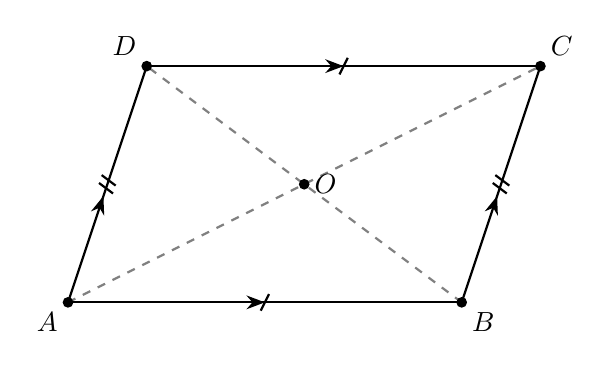
\begin{tikzpicture}[scale=1.0, thick,
  tickone/.style={postaction={decorate, decoration={markings,
    mark=at position 0.5 with {\draw (-1.5pt,-3pt) -- (1.5pt,3pt);}}}},
  ticktwo/.style={postaction={decorate, decoration={markings,
    mark=at position 0.5 with {\draw (-2.5pt,-3pt) -- (-0.5pt,3pt);
                               \draw (0.5pt,-3pt)  -- (2.5pt,3pt);}}}},
  arrowone/.style={postaction={decorate, decoration={markings,
    mark=at position 0.5 with {\arrow{Stealth}}}}},
  arrowtwo/.style={postaction={decorate, decoration={markings,
    mark=at position 0.45 with {\arrow{Stealth}};
    mark=at position 0.55 with {\arrow{Stealth}}}}},
]
  \coordinate (A) at (0,0);
  \coordinate (B) at (5,0);
  \coordinate (C) at (6,3);
  \coordinate (D) at (1,3);
  \coordinate (O) at ($(A)!0.5!(C)$);
  \draw[tickone, arrowone] (A) -- (B);
  \draw[tickone, arrowone] (D) -- (C);
  \draw[ticktwo, arrowtwo] (A) -- (D);
  \draw[ticktwo, arrowtwo] (B) -- (C);
  \draw[gray, dashed] (A) -- (C);
  \draw[gray, dashed] (B) -- (D);
  \filldraw (O) circle (1.5pt);
  \foreach \pt in {A,B,C,D} \filldraw (\pt) circle (1.5pt);
  \node[below left]  at (A) {$A$};
  \node[below right] at (B) {$B$};
  \node[above right] at (C) {$C$};
  \node[above left]  at (D) {$D$};
  \node[right] at (O) {$O$};
\end{tikzpicture}
\end{document}
